% !TEX root = ../main.tex
\begin{figure}[t]
    \centering
    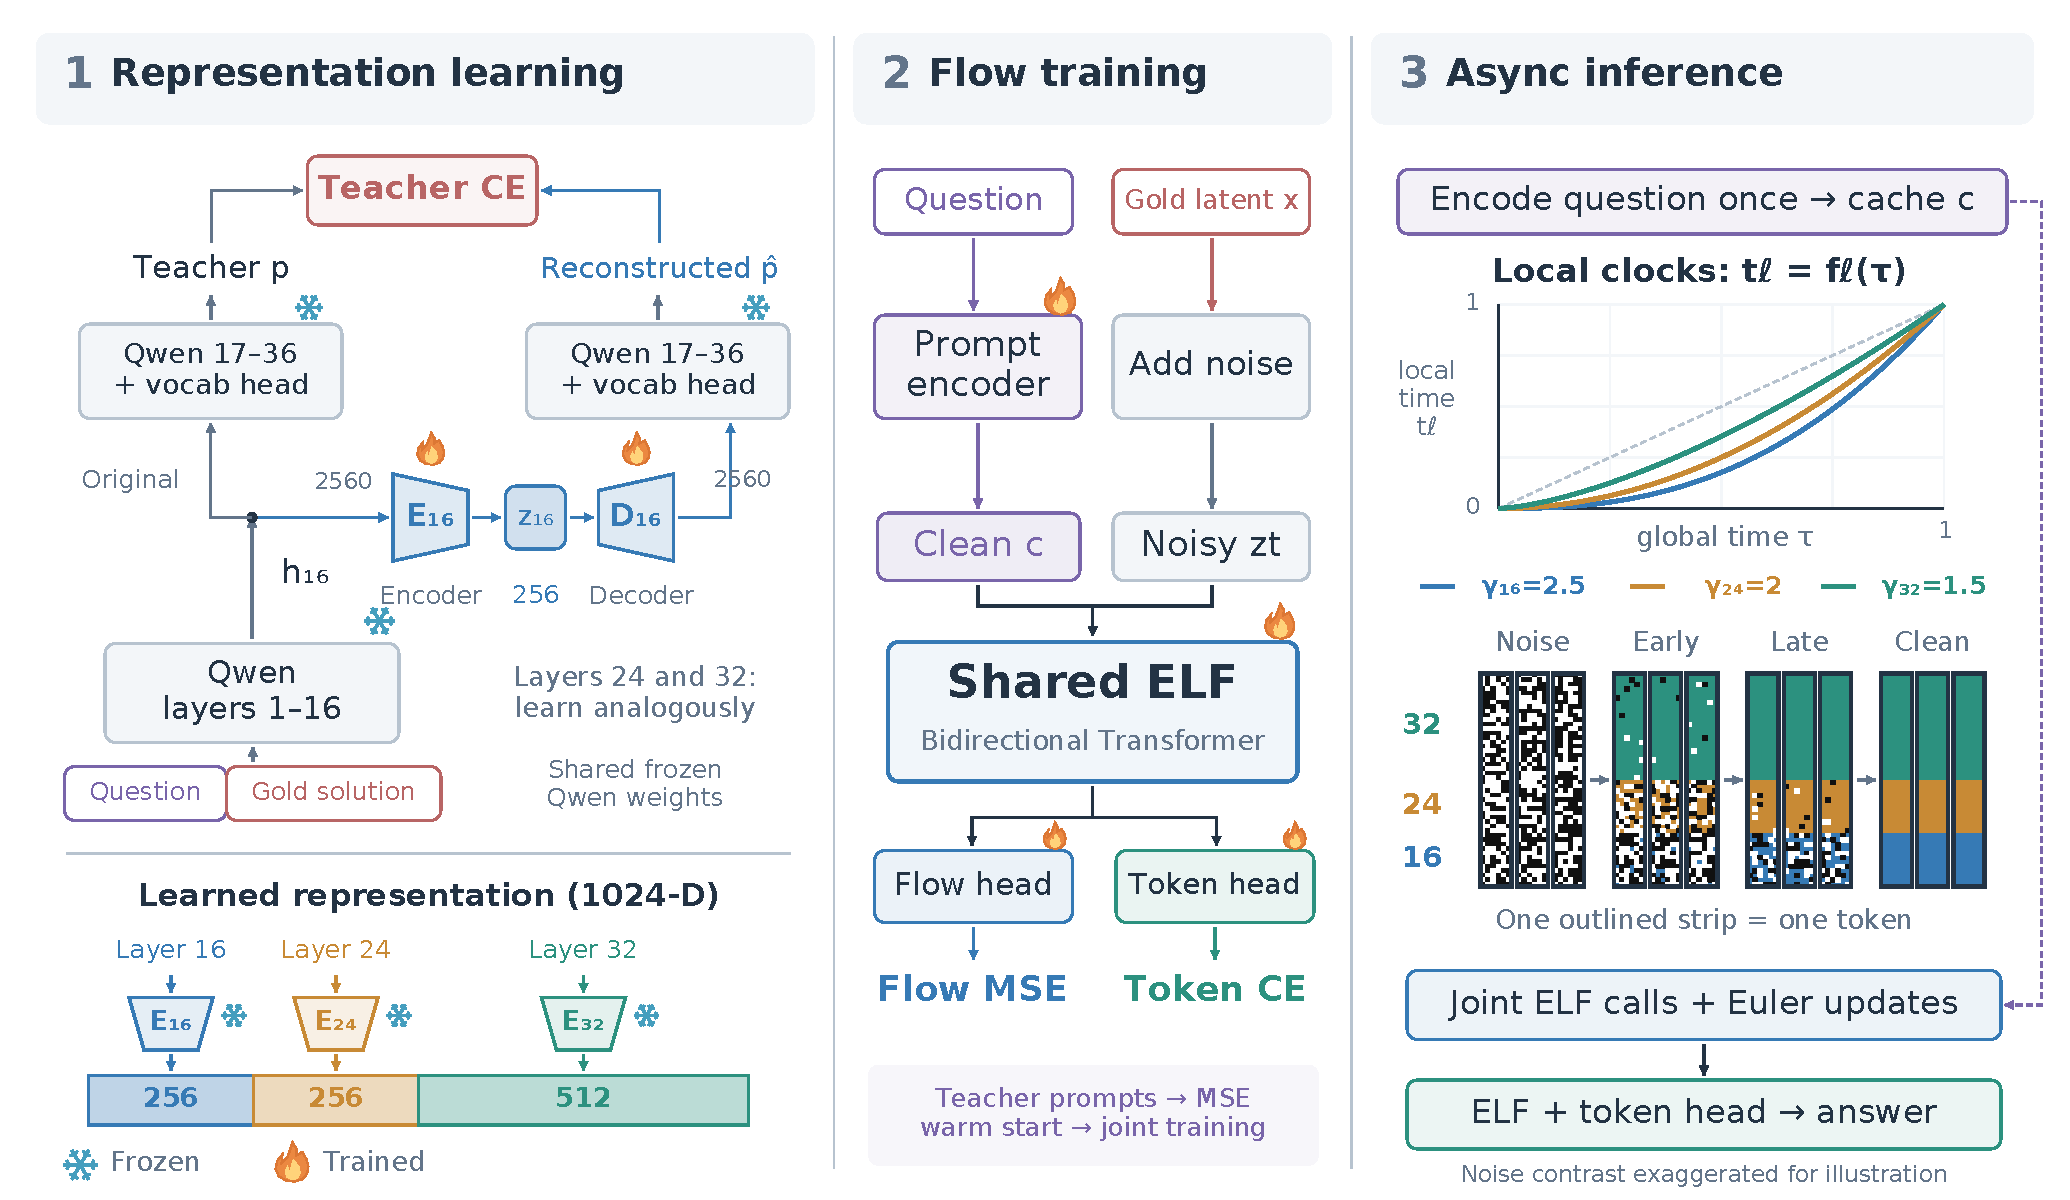
\includegraphics[width=\textwidth]{figures/pipeline_overview_v4.pdf}
    \caption{\textbf{A continuous-diffusion reasoning pipeline.}
    \textbf{Left:} The layer-16 example compares clean teacher predictions $p$ with predictions $\hat p$ after encoding and reconstructing assistant activations. Teacher cross-entropy trains $E_{16}$ and $D_{16}$ through the frozen Qwen suffix. Layers 24 and 32 are learned analogously; the three encoders are then frozen and their 256/256/512-dimensional outputs concatenated (bottom). Covariance whitening is incorporated in the encoder parameterization and omitted from the schematic. Snowflakes and flames denote frozen and trained components.
    \textbf{Center:} A shared bidirectional ELF backbone supports flow matching and token-decoding CE. Training begins with Qwen prompt features, then introduces an MSE-trained question encoder for joint adaptation. The prompt remains clean while answer latents are corrupted.
    \textbf{Right:} At inference, the question is encoded once. All three representation groups pass through ELF jointly, with local clocks $t_\ell=f_\ell(\tau)=\tau^{\gamma_\ell}$ and $(\gamma_{16},\gamma_{24},\gamma_{32})=(2.5,2,1.5)$. Each bold vertical outline encloses one token; solid colors identify layer groups and black-and-white static illustrates noise. The schematic states exaggerate the separation between groups for visibility; the clock curves show the actual schedule. A terminal ELF/token-head call decodes the answer in parallel.}
    \label{fig:pipelineoverview}
\end{figure}
